\documentclass[11pt]{article}

\usepackage[T1]{fontenc}
\usepackage[polish]{babel}
\usepackage[utf8]{inputenc}
\usepackage{lmodern}
\usepackage{graphicx}
\selectlanguage{polish}



\begin{document}
\title{ \textbf{Sprawozdanie} \protect\\ Problem transportowy wielu produktów}
\author{Bartosz Wlazło, Przemysław Jekiel}
\maketitle
\pagenumbering{arabic}

\newpage 


\section{Wstęp}

\subsection{Problematyka}

Celem niniejszego ćwiczenia było rozwiązanie problemu transportowego wielu produktów. 

\subsection{Cel ćwiczenia}

Po wykonaniu tego ćwiczenia powinniśmy opanować importowanie danych (przy użyciu biblioteki Pandas), umieć skonfigurować i poprawnie wyświetlić dane w cześci frontend oraz umieć korzystać z biblioteki opymalizacyjnej pyscipopt. 

\subsection{Przyjęty przypadek użycia}

Osoba X prowadzi sieć sklepów spożywczych. Największe koszty, które ponosi firma są związane z transportem produków z magazynów do sklepów. W celu obniżenia ich udała się ona do firmy OPTTech w celu opracowania narzędzia do planowania tras i ilości zabieranych produktów.

\section{Narzędzia}
Do obliczeń oraz wizualizacji danych i wyników zostały użyte następujące narzędzia:
\begin{itemize}
	\item Python - mikroframework Flask - realizacja zadania frontend tj. wizualizacja danych i wyników oraz GUI użytkownika
	\item Python - biblioteka Pyscipopt - realizacja zadania backend tj. stworzenia modelu problemu i obliczenia wyniku
	\item Python - biblioteka Pandas - realizacja zadania backend tj. import i obróbka importowanych z pliku bazowodanego danych	
\end{itemize}
\section{Założenia projektowe}
\subsection{Uproszczające}
W celu szybszej pracy kody próbka danych został ograniczona do:
\begin{itemize}
	\item 5 sklepów 
	\item 3 magazynów
	\item 4 typów produktów
	\item nieskończonej liczby środków transportu 
	\item wartości ograniczeń są wyrażone w liczbach całkowitych 
\end{itemize}

Zostało także przyjęte uproszczenie iż każdy produkt jest magazowany w tej samej liczbie.

\subsection{Przyjęte zmienne}
\begin{itemize}
	\item $\displaystyle I$ - zbiór sklepów \textit{i}
	\item $\displaystyle i$ - \textit{t}-ty sklep 
    \item $\displaystyle J$ - zbiór magazynów \textit{j}
	\item $\displaystyle j$ - \textit{j}-ty magazyn 
	\item $\displaystyle K$ - zbiór produktów \textit{k}
	\item $\displaystyle k$ - \textit{k}-ty produkt
	\item $\displaystyle M_j$ - pojemność \textit{j}-tego magazynu 
	\item $\displaystyle c_{i,j,k}$ - koszt dostawy do \textit{i}-tego sklepu z \textit{j}-tego magazynu \textit{k}-tego produktu 
	\item $\displaystyle d_{i,k}$ - zapotrzebowanie \textit{i}-tego sklepu na \textit{k}-ty produkt
\end{itemize}

\subsection{Szukane}
$\displaystyle x_{i,j,k}$ - ilość wysłanych sztuk produktu \textit{k} do \textit{i} sklepu z \textit{j} magazynu
\subsection{Model matematyczny}
\subsubsection{Funkcja celu}
\begin{center}
$\displaystyle minimize \sum_{i=1}^{n}\sum_{j=1}^{m}\sum_{k=1}^{K} c_{i,j,k}*x_{i,j,k}$
\end{center}
\subsubsection{Ograniczenia}	
	\begin{enumerate}
	\item $\displaystyle \sum_{j=1}^{m} x_{i,j,k}=d_{i,k}$ dla i=1,...,n, k=1,...,K
	\item $\displaystyle \sum_{i=1}^{n}\sum_{k=1}^{K}x_{i,j,k}\le M_j$ dla j=1,...,m
	\item $\displaystyle x_{i,j,k}\ge 0$ dla i=1,...,n, j=1,...,m, k=1,...,K
	\end{enumerate}

\section{Założenia projektowe}
\subsection{Dane ograniczeń}
\subsubsection{\textit{Pojemności magazynów}}
\begin{center}
	\begin{tabular}{ |c|c| } 
		\hline
		 Magazyn & Pojemność\\
		\hline
		Magazyn 1 & 3000  \\ 
		\hline
		Magazyn 2 & 3000  \\ 
		\hline
		Magazyn 3 & 3000  \\ 
		\hline
	\end{tabular}
\end{center}

\subsubsection{\textit{Dostępność produktów w danych magazynach}}
\begin{center}
	\begin{tabular}{ |c|c| } 
		\hline
		Magazyn & Produkt \\
		\hline
		Magazyn 1 & 2, 4  \\ 
		\hline
		Magazyn 2 & 1, 2, 3  \\ 
		\hline
		Magazyn 3 & 2, 3, 4  \\ 
		\hline
	\end{tabular}
\end{center}

\subsection{Dane}

\subsubsection{\textit{Zapotrzebowanie sklepów na dany produkt}}
\begin{center}
	\begin{tabular}{ |c|c|c | } 
		\hline
		Magazyn & Produkt & Zapotrzebowanie\\
		\hline
		Sklep 1 & 1 & 80\\ 
		\hline
		Sklep 1 & 2 & 85\\ 
		\hline
		Sklep 1 & 3 & 300\\ 
		\hline
		Sklep 1 & 4 & 6\\ 
		\hline
		Sklep 2 & 1 & 270\\ 
		\hline
		Sklep 2 & 2 & 160\\ 
		\hline
		Sklep 2 & 3 & 400\\ 
		\hline
		Sklep 2 & 4 & 7\\ 
		\hline
		Sklep 3 & 1 & 250\\ 
		\hline
		Sklep 3 & 2 & 130\\ 
		\hline
		Sklep 3 & 3 & 350\\ 
		\hline
		Sklep 3 & 4 & 4\\ 
		\hline
		Sklep 4 & 1 & 160\\ 
		\hline
		Sklep 4 & 2 & 60\\ 
		\hline
		Sklep 4 & 3 & 200\\ 
		\hline
		Sklep 4 & 4 & 3\\ 
		\hline
		Sklep 5 & 1 & 180\\ 
		\hline
		Sklep 5 & 2 & 40\\ 
		\hline
		Sklep 5 & 3 & 150\\ 
		\hline
		Sklep 5 & 4 & 5\\ 
		\hline
	\end{tabular}
\end{center}

\subsubsection{\textit{Wagi produktów}}
\begin{center}
	\begin{tabular}{ |c|c| } 
		\hline
		Produkt & Waga \\
		\hline
		Produkt 1 & 5  \\ 
		\hline
		Produkt 2 & 2  \\ 
		\hline
		Produkt 3 & 3  \\ 
		\hline
		Produkt 4 & 4  \\ 
		\hline
	\end{tabular}
\end{center}

\subsubsection{\textit{Koszt dostawy do danego sklepu z magazynu}}
\begin{center}
	\begin{tabular}{ |c|c|c | } 
		\hline
		Sklep & Magazyn & Koszt\\
		\hline
		Sklep 1 & Magazyn 1	& 4 \\ 
		\hline
		Sklep 2& 	Magazyn 1& 	5\\ 
		\hline
		Sklep 3	& Magazyn 1	& 6\\ 
		\hline
		Sklep 4	& Magazyn 1& 	8\\ 
		\hline
		Sklep 5& 	Magazyn 1& 	10\\ 
		\hline
		Sklep 1& 	Magazyn 2& 	6\\ 
		\hline
		Sklep 2& 	Magazyn 2& 	4\\ 
		\hline
		Sklep 3& 	Magazyn 2& 	3\\ 
		\hline
		Sklep 4	& Magazyn 2& 	5\\ 
		\hline
		Sklep 5	& Magazyn 2	& 8\\ 
		\hline
		Sklep 1& 	Magazyn 3& 	9\\ 
		\hline
		Sklep 2& 	Magazyn 3& 	7\\ 
		\hline
		Sklep 3& 	Magazyn 3& 	4\\ 
		\hline
		Sklep 4	& Magazyn 3& 	3\\ 
		\hline
		Sklep 5	& Magazyn 3	& 4\\ 
		\hline
	\end{tabular}
\end{center}
\newpage

\section{Interfejs użytkownika}
\subsection{Widok strony głównej}
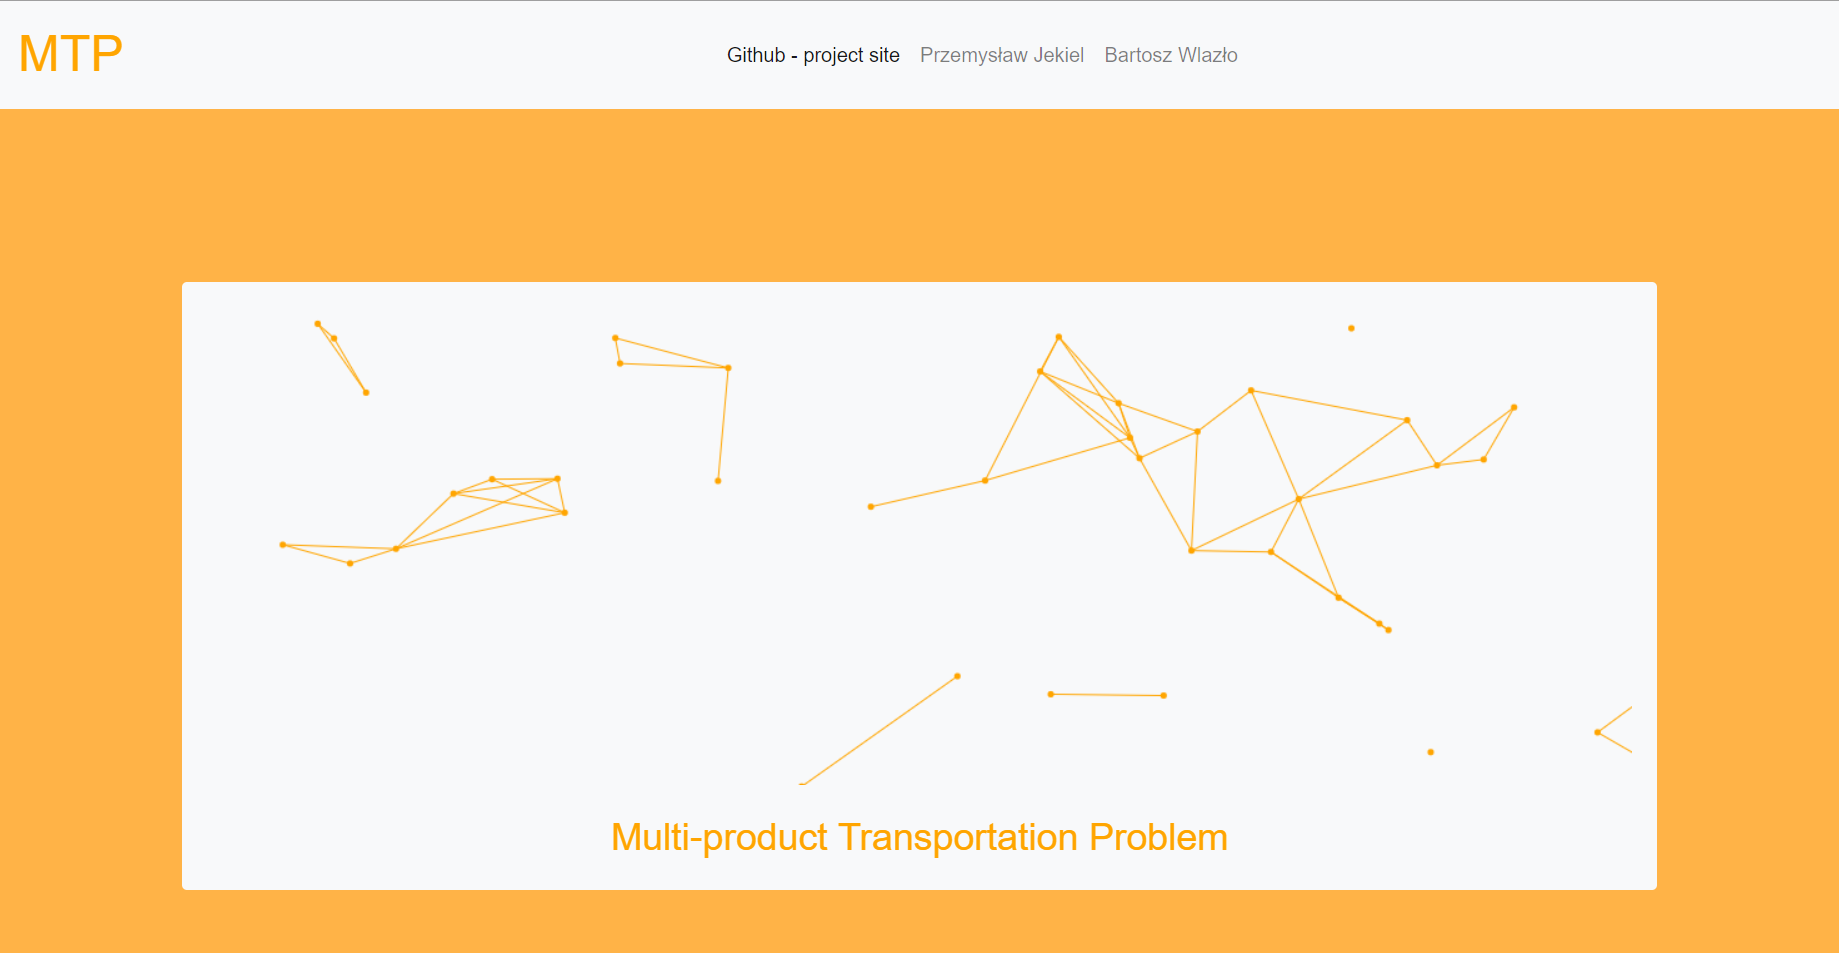
\includegraphics[width=\textwidth,height=\textheight,keepaspectratio]{1.png}
\subsection{Widok strony z wynikami}
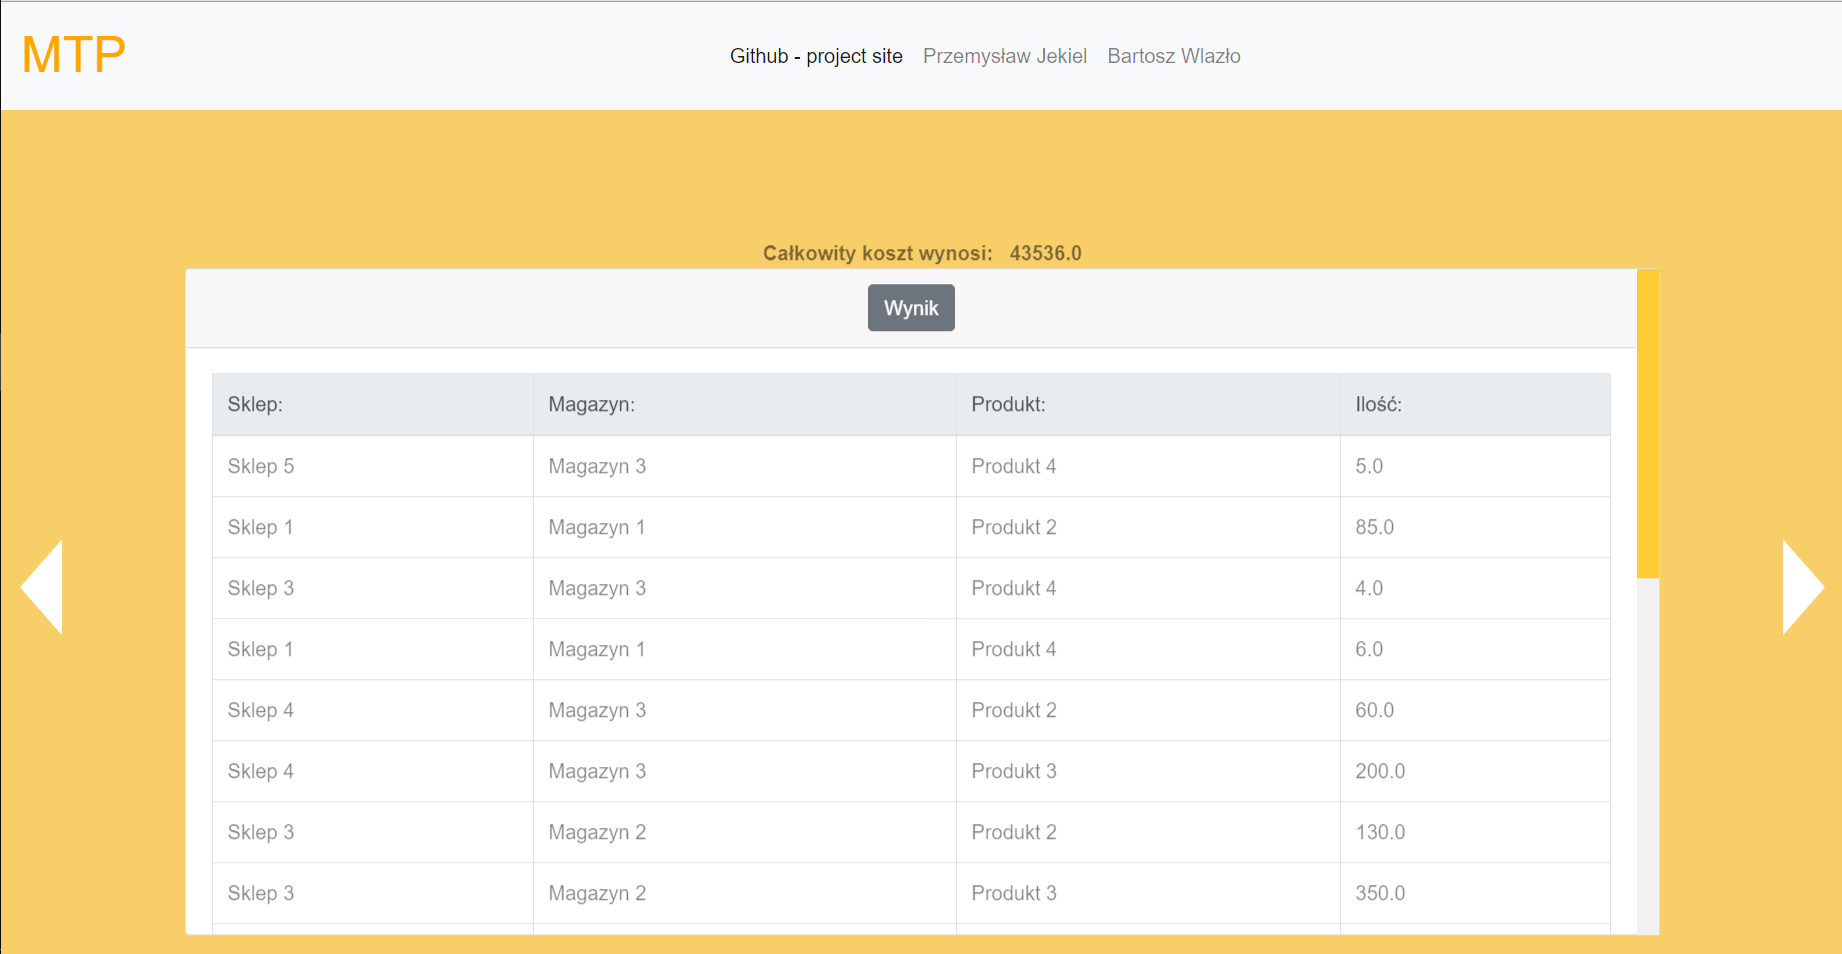
\includegraphics[width=\textwidth,height=\textheight,keepaspectratio]{2.png}
\section{Wynik}
Dla podanych danych całkowity koszt wynosi:   43536.0\\
\begin{center}
Tabela z wynikami
\end{center}
\begin{center}
	\begin{tabular}{ |c|c|c|c| } 
		\hline
		Sklep	& Magazyn	& Produkt	& Ilość sztuk\\
		\hline
		Sklep 5	& Magazyn 3	& Produkt 4	& 5.0\\
		\hline
		Sklep 1	& Magazyn 1	& Produkt 2	& 85.0\\
		\hline
		Sklep 3	& Magazyn 3	& Produkt 4	& 4.0\\
		\hline
		Sklep 1	& Magazyn 1	& Produkt 4	& 6.0\\
		\hline
		Sklep 4	& Magazyn 3	& Produkt 2	& 60.0\\
		\hline
		Sklep 4	& Magazyn 3	& Produkt 3	& 200.0\\
		\hline
		Sklep 3	& Magazyn 2	& Produkt 2	& 130.0\\
		\hline
		Sklep 3	& Magazyn 2	& Produkt 3	& 350.0\\
		\hline
		Sklep 2	& Magazyn 2	& Produkt 1	& 270.0\\
		\hline
		Sklep 4	& Magazyn 2	& Produkt 1	& 160.0\\
		\hline
		Sklep 2	& Magazyn 1	& Produkt 4	& 7.0\\
		\hline
		Sklep 2	& Magazyn 2	& Produkt 3	& 400.0\\
		\hline
		Sklep 2	& Magazyn 2	& Produkt 2	& 160.0\\
		\hline
		Sklep 5	& Magazyn 2	& Produkt 1	& 180.0\\
		\hline
		Sklep 3	& Magazyn 2	& Produkt 1	& 250.0\\
		\hline
		Sklep 1	& Magazyn 2	& Produkt 3	& 300.0\\
		\hline
		Sklep 5	& Magazyn 3	& Produkt 3	& 150.0\\
		\hline
		Sklep 5	& Magazyn 3	& Produkt 2	& 40.0\\
		\hline
		Sklep 4	& Magazyn 3	& Produkt 4	& 3.0\\
		\hline
		Sklep 1	& Magazyn 2	& Produkt 1	& 80.0\\
		\hline
	\end{tabular}
\end{center}
\section{Analiza otrzymanych wyników}
Analiza wyników jest trudna do osiągnięcia ze względu na charakter zadania. Porównanie z wynikami rzeczywistymi jest niemożliwe ze względu na brak dostępu do takowych. Model został wykonany na czysto teoretycznym wycinku rzeczywistości.
\section{Wnioski}
Zbudowanie modelu w skali pozwala na uniknięcie kosztów związanych z wykonywaniem testów w rzeczywistym środowisku. Oszczędzane są również inne zasoby takie jak chociażby czas.
\\Dzięki temu ćwiczeniu opanowaliśmy wiedzę z zakresu:
\begin{itemize}
	\item Frontend - konfiguracji oraz obsługi mikroframeworku flask w języku programowania Python
	\item Backend - operacji na danych dzięki obsłudze biblioteki Pandas w języku programowania Python
	\item Backend - optymalizacji dzięki bibliotece pyscipopt w języku programowania Python
	\item tworzenia plików teskstowych z wykorzytaniem LaTeX 
\end{itemize}

\newpage 

\section{Kod}
Kod jest dostępny ws repozytorium: 
https://github.com/pj30/Projekt-MMPPiZ
\end{document}
